% file containing the general overview for the design spec
% Subsections: goals, dev plans, timeline, use cases/flowcharts
% Domanic
\documentclass{article}
\usepackage{ragged2e}
\usepackage{tikz}
\usetikzlibrary{shapes.geometric, arrows}
\tikzstyle{startstop} = [rectangle, rounded corners, minimum width=3cm, minimum height=1cm, text centered, text width=3cm, draw=black, fill=red!30]
\tikzstyle{io} = [trapezium, trapezium left angle=70, trapezium right angle=110, minimum width=3cm, minimum height=1cm, text centered, text width=3cm, draw=black, fill=blue!30]
\tikzstyle{process} = [rectangle, minimum width=3cm, minimum height=1cm, text centered, text width=3cm, draw=black, fill=orange!30]
\tikzstyle{decision} = [diamond, minimum width=3cm, minimum height=1cm, text centered, text width=1.5cm, draw=black, fill=green!30]
\tikzstyle{arrow} = [thick, ->, >=stealth]
\begin{document}
\section{General}
This design spec is to outline and specify the details of our team's Tower of Light project. Throughout this document our team will detail how we have decided to develop this application, starting with our goals and getting down to functionality and features.
\subsection{Goals}
Our team's main goal is the completion of our Tower of Light application before the assigned due date, which is currently undecided. This can be achieved through the completion of mini-goals that when completed will result in a finished product.
	\begin{itemize}
		\item Our first goal should be the completed design of our application, which is partially achieved through the creation of this document. This goal is necessary for the creation of the 				project to go smoothly.
		\item After we have a finished design the next goal will be the creation of a simple form of our application which will be version 0.1. This version should only contain the minimum core 				functionality for the Tower of Lights application detailed in this document.
		\item Once our team has a working version 0.1 our next goal will be to include as many additional features that we can get working correctly before the due date. The completion of this goal will result in achieving our overall goal.
	\end{itemize}
\subsection{Development Plans}
We plan to develop our application through the specified goals and time line. Each week we will set a task for our team to finish until the project is complete. Given time constraints this will be a quick process with multiple meetings to discuss how to complete these weekly tasks. 
\subsection{Timeline}
This time line is a rough estimate of each week's tasks that will be completed to finish our Tower of Lights application. It has yet to be fully reviewed by the team and is subject to change.
	\begin{itemize}
		\item \textbf{Week 1 (10/26 - 11/2)} The first week will be dedicated to completing the rough draft of this Design Specification. 
		\item \textbf{Week 2 (11/2 - 11/9)} Since the Design of a program is crucial this week will also be used to finish the design specification in greater detail.
		\item \textbf{Week 3 (11/9 - 11/16)} Once the overall design of the application is finished we will create the interface we decided with Qt.
		\item \textbf{Week 4 (11/16 - 11/23)} With a completed interface our team can start to program in the core functionality for the application.
		\item \textbf{Week 5 (11/23 - 11/30)} It will probably take some extra time to get the base program working so this week will also be assigned to finishing the first version, although 				can be used for additional features if ahead of time.
		\item \textbf{Week 6 (11/30 - 12/7)} At this point we should have some working version and from here we can continue adding features till the due date.
		\item \textbf{Week 7 (12/7 - 12/14)} This will be the absolute last week (possibly) to finish our application with additional features.
	\end{itemize}
\subsection{Flowchart}
This section is used to display several flowcharts where each is a representation for how a user will interact with a section of the program. These flowcharts will represent how we want the core functionality of the application to function.
\subsubsection{User interaction with the toolbox}
\centering
	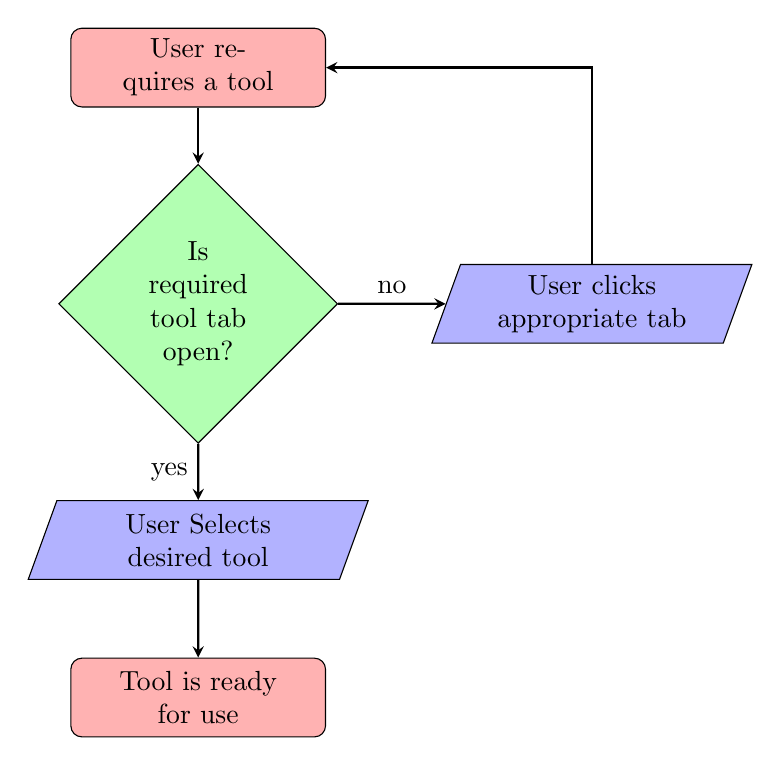
\begin{tikzpicture}[node distance=2cm]
		\node (start) [startstop] {User requires a tool};
		\node (dec1) [decision, below of=start, yshift=-1cm] {Is required tool tab open?};
		\node (in1) [io, right of=dec1, xshift=3cm] {User clicks appropriate tab};
		\node (in2) [io, below of=dec1, yshift=-1cm] {User Selects desired tool};
		\node (stop) [startstop, below of=in2] {Tool is ready for use};
		\draw [arrow] (start) -- (dec1);
		\draw [arrow] (in2) -- (stop);
		\draw [arrow] (dec1) -- node[anchor=south] {no} (in1);
		\draw [arrow] (dec1) -- node[anchor=east] {yes} (in2);
		\draw [arrow] (in1) |- (start);
	\end{tikzpicture}
	\begin{flushleft}
		\subsubsection{User interaction with the editor}
	\end{flushleft}
		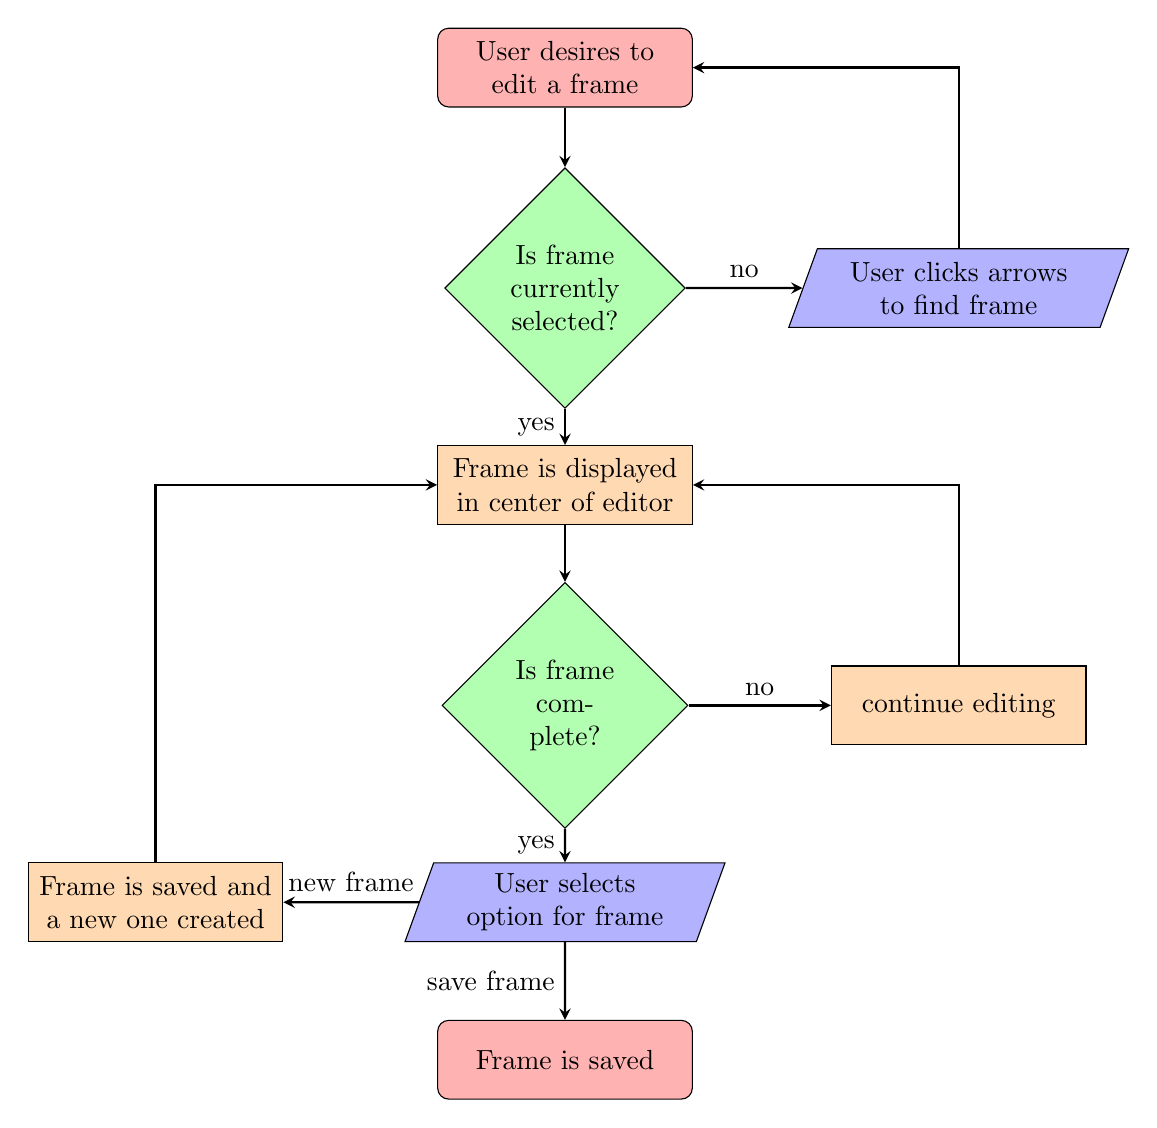
\begin{tikzpicture}[node distance=2cm]
			\node (start) [startstop] {User desires to edit a frame};
			\node (dec1) [decision, below of=start, yshift=-.8cm] {Is frame currently selected?};
			\node (in1) [io, right of=dec1, xshift=3cm] {User clicks arrows to find frame};
			\node (proc1) [process, below of =dec1, yshift=-0.5cm] {Frame is displayed in center of editor};
			\node (dec2) [decision, below of=proc1, yshift=-0.8cm] {Is frame complete?};
			\node (proc2) [process, right of=dec2, xshift=3cm] {continue editing};
			\node (in2) [io, below of=dec2, yshift=-0.5cm] {User selects option for frame};
			\node (proc3) [process, left of=in2, xshift=-3.2cm] {Frame is saved and a new one created};
			\node (stop) [startstop, below of=in2] {Frame is saved};
			\draw [arrow] (start) -- (dec1);
			\draw [arrow] (dec1) -- node[anchor=south] {no} (in1);
			\draw [arrow] (dec1) -- node[anchor=east] {yes} (proc1);
			\draw [arrow] (in1) |- (start);
			\draw [arrow] (proc1) -- (dec2);
			\draw [arrow] (dec2) -- node[anchor=south] {no} (proc2);
			\draw [arrow] (dec2) -- node[anchor=east] {yes} (in2);
			\draw [arrow] (proc2) |- (proc1);
			\draw [arrow] (in2) -- node[anchor=south] {new frame} (proc3); 
			\draw [arrow] (proc3) |- (proc1);
			\draw [arrow] (in2) -- node[anchor=east] {save frame} (stop);
		\end{tikzpicture}
\end{document}